本章では, 本研究での予備的なプロセスを述べる



%(波及効果)
%非流暢性によって場面の違いを数値化する(場面の違いを非流暢性に置き換える)(波及効果)さまざまな場面での比較、検討ができるようになる

%使用データ
%非流暢性のアノテーション

%非流暢性と対話場面との関係について(親密さの違い、話し相手男女の違い)(結果)
%個人間の非流暢性の変化について(考察)

\subsection{予備的なプロセスについて}
%予備的なプロセスの背景
 そもそもの問題として日常対話コーパスを扱ううときに、対話場面の違いをどのように体系化することができるのかという問題がある。日常の中の対話場面での関係の変化として親密度の変化が生じることが考えられる。
 先行研究の中で、音声に付随する書き起こしテキストに対して、speaking styleの自動推定のために、明瞭さ・親しさ・社会階層の3尺度を用いて推定を行なっている\cite{shen}。書き言葉に対して親密度の変化が重要であるのと同様に、話し言葉においても親密度の変化は重要な要素であるといえる。
%予備的なプロセスの目的
親密度が異なる場面で非流暢性の特徴がどのように変化するのかを調べる。
%予備的なプロセスの波及効果
非流暢性の特徴を明らかにすることで、対話場面の違いを非流暢性の特徴から分類することができると考えられる。また、非流暢性によって場面の違いを数値化することで、多種多様な場面を非流暢性という観点から比較検討することができるようになると考えられる。

\subsection{使用データ}\label{data}
 使用データは、同研究室で収集された『新入生対話コーパス』(FDC)\cite{FDC}の2011年の対話を使用する。本コーパスは、比較的初対面である大学生二名が行った対話と半年後に同じ二名で行った対話が収録されている。2011年の対話を今回の分析に使用した理由は、1度目の対話が完全に初対面であるためである。分析に用いたデータは、FDCから男性と男性の対話2組、女性と男性の対話2組、合計8対話である。FAOMFUとFAOMNAは男性対女性の対話であり、MAKMTKとMTKMTTは男性対男性の対話である。

\subsection{非流暢性のアノテーション}
アノテーションには、伝らの非流暢性の分類を使用した。以下にその分類を示す。音韻の引き伸ばしとは、発話の切れ目において母音を持続して発話することである。フィラーとは、発話における無意味語のことである。語の中断とは、ある単語の途中で言葉を言い止めることである。語句の繰り返しは、同じ単語を複数回繰り返すことである。語の言い直しとは、一度発話した単語を違う単語に言い直すことである\cite{den}。
なお、フィラーの分類は『日本語話し言葉コーパス』(CSJ)の書き起こし基準に準ずる\cite{hanashi}。

\subsection{結果}
 対話に現れる非流暢性の出現頻度を図\ref{disfluency}に示す。男性対女性の対話の半年前と半年後の非流暢性の出現頻度を図\ref{FAOMFU}、図\ref{FAOMNA}に、男性対男性の対話の半年前と半年後の非流暢性の出現頻度を図\ref{MAKMTK}、図\ref{MTKMTT}に示す。
\begin{figure}[htbp]
    \begin{tabular}{cc}
      \begin{minipage}[t]{0.45\hsize}
        \centering
        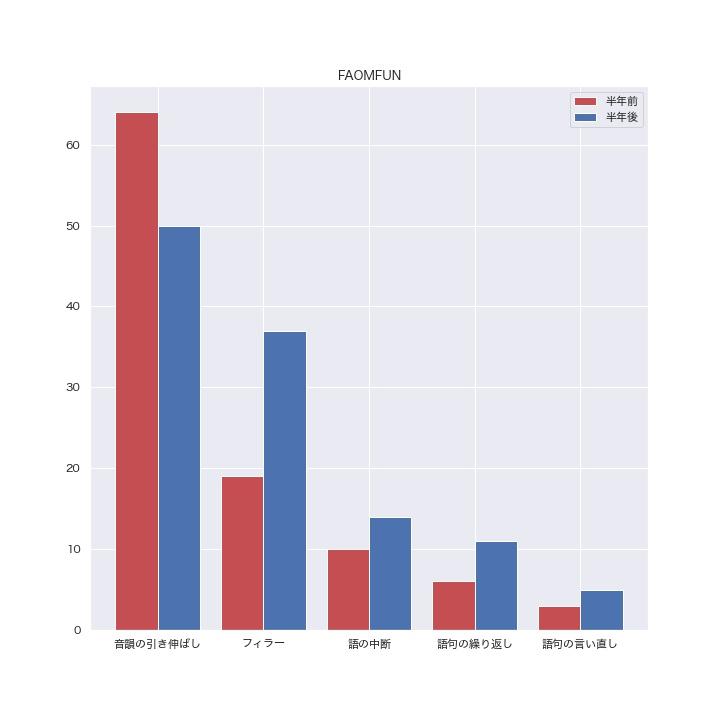
\includegraphics[keepaspectratio, scale=0.3]{figures/FAOMFUN.jpg}
        \subcaption{FAOMFU}
        \label{FAOMFU}
      \end{minipage} &
      \begin{minipage}[t]{0.45\hsize}
        \centering
        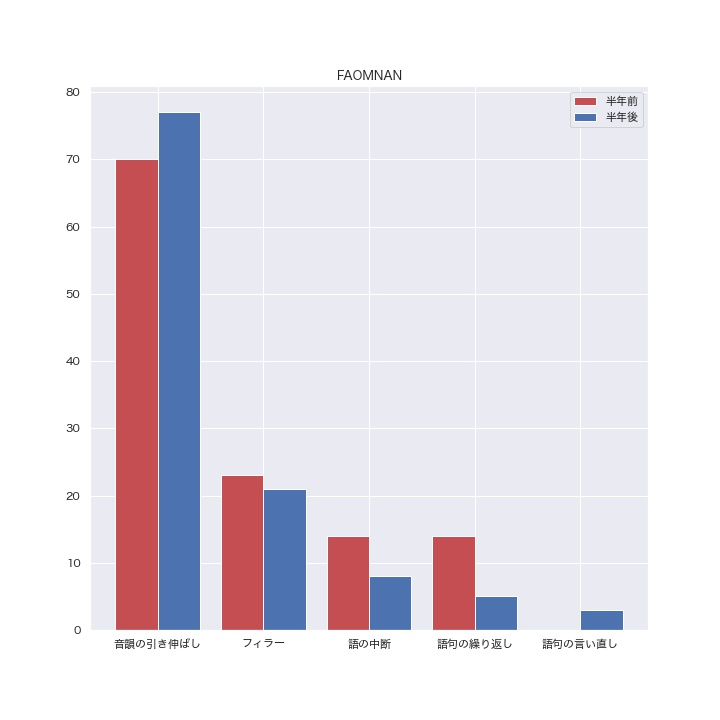
\includegraphics[keepaspectratio, scale=0.3]{figures/FAOMNAN.jpg}
        \subcaption{FAOMNA}
        \label{FAOMNA}
      \end{minipage} \\
   
      \begin{minipage}[t]{0.45\hsize}
        \centering
        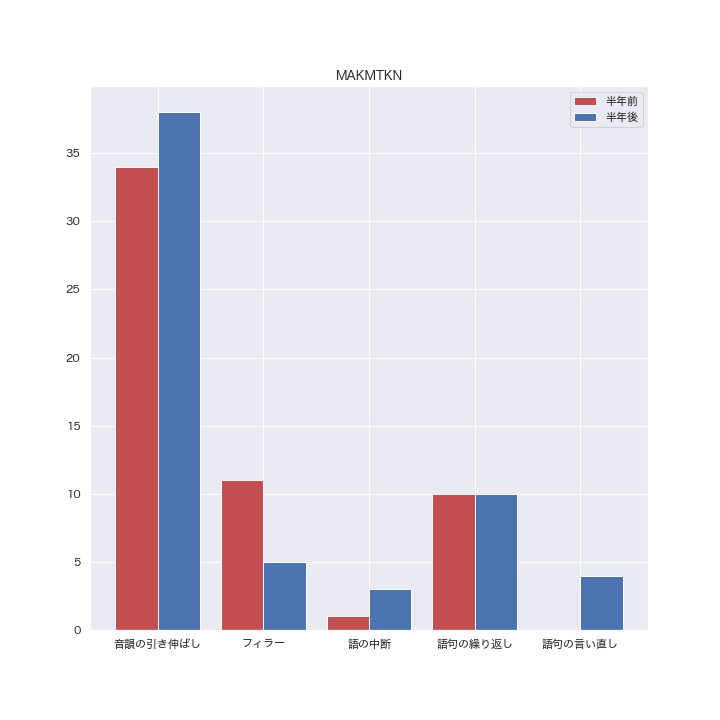
\includegraphics[keepaspectratio, scale=0.3]{figures/MAKMTKN.jpg}
        \subcaption{MAKMTK}
        \label{MAKMTK}
      \end{minipage} &
      \begin{minipage}[t]{0.45\hsize}
        \centering
        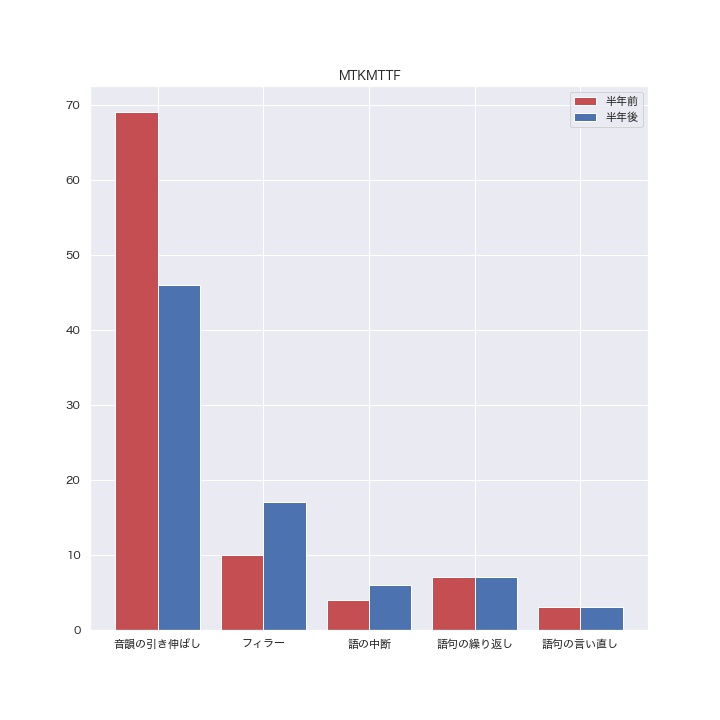
\includegraphics[keepaspectratio, scale=0.3]{figures/MTKMTTF.jpg}
        \subcaption{MTKMTT}
        \label{MTKMTT}
      \end{minipage} 
    \end{tabular}
     \caption{対話に出現する非流暢性の半年前と半年後の出現頻度}
     \label{disfluency}
  \end{figure}

\newpage

\subsection{考察}
半年前と半年後の親密度の変化によって、非流暢性が一様に変化するという結果は得られなかった。しかし、非流暢性の出現頻度は個人差の影響が大きいことから、個人に着目することでどのような特徴があるのかについて明らかにできると考える。また、男性対女性の対話と男性対男性の対話に分けて分析することで、非流暢性の変化の傾向を知ることができると考える。

%個人間の非流暢性の変化について(考察)

